% !TEX root = ../main.tex
%
\chapter{Vorgeschlagenes Wissensgraph\-konstruktions\-verfahren}%
\label{sec:text2kg}

Auf Basis der vorgestellten Konzeptgraphen, CoreNLP und PSL wird im folgenden Kapitel ein Verfahren für die online Konstruktion eines Wissensgraphen aus natürlichsprachlichen Textnachrichten aufgebaut.
Der Fokus liegt dabei primär auf der generellen Architektur des Verfahrens.
Das Resultat ist also als Proof-of-Concept zu verstehen, auf dessen Basis praxistaugliche Systeme konzipiert werden können.

\begin{figure}[h]
	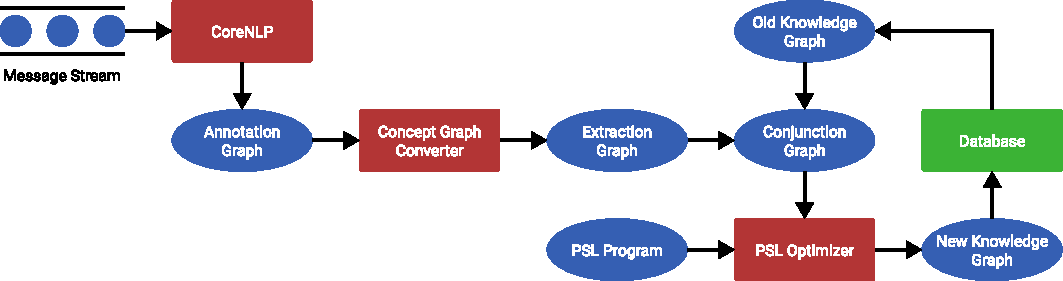
\includegraphics[width=\textwidth]{gfx/text2kg/architecture.pdf}
	\caption{Grobes Architekturdiagramm der Konstruktionspipeline}\label{fig:text2kg:architecture}
\end{figure}
Das im Folgenden vorgestellte Verfahren folgt einem dreistufigen Pipeline-Modell:
\begin{enumerate}
	\item Mittels CoreNLP wird eine eintreffende Textnachricht in einen Abhängigkeitsgraphen transformiert.
	\item Der resultierende Abhängigkeitsgraph wird in einen sog.\ Extraktionsgraphen umgewandelt.
		Hierbei handelt es sich um einen Konzeptgraphen, der den Inhalt der Nachricht formal repräsentiert.
	\item Der Extraktionsgraph wird mit dem bestehenden Wissensgraphen verschmolzen.
		Dies entspricht der Konjuktion der durch die beiden Graphen repräsentierten logischen Ausdrücke.
		Der resultierende Konjunktionsgraph wird als Eingabe für ein PSL-Programm verwendet, welches auf Basis des hinzugekommenen Wissens neue Beziehungen im Wissensgraphen inferiert.
\end{enumerate}
Die Beschreibung dieser Pipeline erfolgt in vier Abschnitten.
In \treft{sec:text2kg:implementation} wird kurz die technische Umsetzung erläutert.
\treft{sec:text2kg:ontology} beschreibt anschließend die Ontologie der konstruierten Wissensgraphen.
Nach diesen strukturellen Betrachtungen wird schließlich in \treft{sec:text2kg:nlp} und \treft{sec:text2kg:psl} die Transformation von Text zu Extraktionsgraph, bzw.\ von Extraktionsgraph zu Wissensgraph beschrieben.

\section{Implementation}%
\label{sec:text2kg:implementation}

Das in den folgenden Abschnitten beschriebene Verfahren wurde im Rahmen dieser Arbeit prototypisch implementiert.
Bei der Wahl der hierfür verwandten Technologien wurde darauf Wert gelegt, dass eine möglichst nahtlose Integration der Komponenten möglich ist.
Sowohl CoreNLP~\cite{CoreNLP} als auch die PSL-Referenzimplementation~\cite{PSL} sind JVM-Bibliotheken.
Diese Arbeit wurde daher ebenfalls für die JVM implementiert, insbesondere weil es zu der PSL-Referenzimplementation keine Alternative gibt und eine Reimplementation von PSL den Rahmen dieser Arbeit gesprengt hätte.

Als JVM-Sprache wurde Clojure gewählt; ein moderner Lisp-1-Dialekt, mit einem Fokus auf funktionale Programmierung, unveränderliche Datenstrukturen und gleichzeitiger Interoperabilität mit objektorientierten Bibliotheken.
Andere JVM-Sprachen, wie z.~B. Java, Scala oder Groovy, wurden ausgeschlossen, da sie sich während des Entwicklungsprozesses als hinderlich erwiesen haben.
Der Hauptgrund hierfür ist, dass CoreNLP bei der Initialisierung diverse Modelle laden muss.
Bei Verwendung eines modernen Desktop-Rechners benötigt dies ca.~20 Sekunden, auf langsamerer Hardware teils mehrere Minuten;
diese Wartezeiten waren ein stark verlangsamender Faktor beim entwickeln.
Da Clojure ein Lisp ist, unterstützt es traditionsgemäß \textit{REPL Driven Development}.
Statt nach jeder Änderung die Anwendung neu zu starten und die Modelle erneut zu laden, kann so lediglich der geänderte Bytecode in den laufenden Prozess injiziert werden;
die geladenen Modelle bleiben dabei im Speicher und die Änderung kann ohne weitere Wartezeit getestet werden.
Durch die Wahl von Clojure konnte die Entwicklung deutlich beschleunigt werden.

\section{Wissensgraphontologie}%
\label{sec:text2kg:ontology}

Bevor Wissensgraphen konstruiert werden können, muss spezifiziert sein, wie genau diese aussehen sollen.
Um komplexe logische Beziehungen ausdrücken zu können, wird die bereits vorgestellte Konzeptgraph-Struktur verwendet.
Dabei bleibt allerdings offen, welche Prädikate vorkommen können und welche Bedeutung sie haben.
Außerdem ist unklar, wie mit Konzeptgraphen modale Aussagen ausgedrückt werden.
Damit aus einem Konzeptgraphen ein Wissensgraph wird, muss eine Ontologie gegeben sein, welche diese offenen Punkte schließt.
Im Folgenden wird beschrieben, wie genau die in dieser Arbeit verwendete Ontologie aufgebaut ist.

\subsection{Verwendete Prädikate}%
\label{sec:text2kg:ontology:pred}

Im ersten Schritt wird geklärt, welche Prädikate in den in dieser Arbeit konstruierten Wissensgraphen vorkommen können.
Es ist nicht sinnvoll beliebige Prädikate zuzulassen, da für eine effiziente maschinelle Weiterverarbeitung der Wissensgraphen, eine Semantik für alle vorkommenden Prädikate definiert sein muss.
Für die Wissensgraphen in dieser Arbeit wird daher eine Menge von fünf Prädikaten verwendet.

\paragraph{Syntax}
Bevor diese Prädikate näher erläutert werden, wird allerdings die Konzeptgraphsyntax leicht modifiziert.
Da alle verwendeten Prädikate entweder unär oder binär sein werden, kann eine kompaktere Notation benutzt werden:
\begin{align}
	\vcenter{\hbox{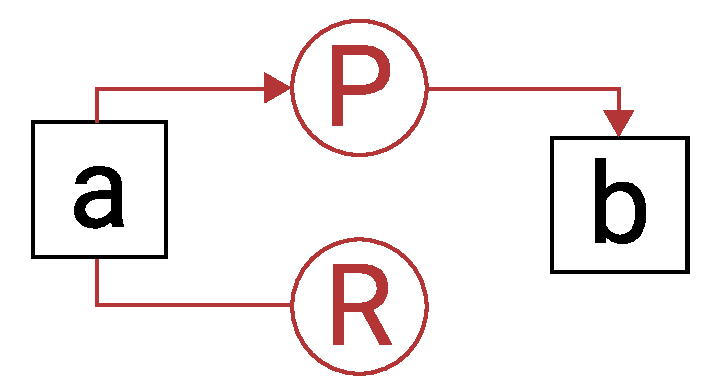
\includegraphics[scale=0.23]{gfx/text2kg/relationNodeAlternativeSyntax1.pdf}}}
	\Leftrightarrow
	\vcenter{\hbox{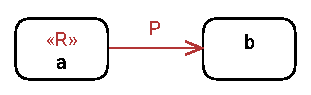
\includegraphics[scale=0.8]{gfx/text2kg/relationNodeAlternativeSyntax2.pdf}}}
\end{align}
Relationsknoten werden nicht mehr dargestellt.
Bei unären Relationen werden die Relationsknotenbezeichner stattdessen mit in die Konzeptknoten geschrieben.
Binäre Relationen werden durch eine bezeichnete Kante zwischen dem ersten und zweiten Argument repräsentiert.

\paragraph{Wissensmodell}
Um eine semantisch konsistente Menge von Wissensgraph-Prädikaten zu definieren, ist es sinnvoll zuvor ein Modell zu definieren, welches den abstrakten Begriff des \textit{Konzeptes} formalisiert.
Konzepte sind das zentrale Syntaxelement in Konzeptgraphen;
ähnlich wie Variablen in der Prädikatenlogik, haben sie jedoch keine inhärente Bedeutung.

Im Folgenden wird ein Konzept $x$ durch eine Eigenschaftsmenge $prop(x) = \{ p_1, \dots, p_n \}$ spezifiziert.
Prädikate die für $x$ gelten bzw.\ nicht gelten, beschreiben Eigenschaften von $prop(x)$.
Es ist unrealistisch $prop(x)$ mittels Prädikaten vollständig zu definieren, da dies gleichbedeutend mit einer exakten formalen Beschreibung jedes beliebigen Konzeptes $x$ wäre.
Das Ziel ist daher stattdessen, die Eigenschaftsmengen von Konzepten in Relation zueinander zu beschreiben.
Der Wissensgraph ist also ein Formalismus zur Beschreibung von Eigenschaften der Eigenschaftsmengen von Konzepten.

\paragraph{Prädikate}
Abhängig davon, welche Eigenschaften erfasst werden sollen, können die zu verwendenden Prädikate stark variieren.
Die für diese Arbeit verwendete Prädikatsmenge hat nicht das Ziel der Vollständigkeit, sondern versucht vielmehr einige wesentliche Eigenschaften natürlichsprachlicher Aussagen zu erfassen.
Gemäß dieser Prämisse wurden fünf Wissensgraph-Prädikate definiert.
\begin{enumerate}
	\item \textbf{$label \subseteq \text{concept} \times \text{string}$:}
		Das $label$-Prädikat wird benutzt, um den Bezeichner eines Konzeptes zu repräsentieren.
		Jedes Konzept hat höchstens einen Bezeichner.
		Da Konzepte aus natürlichsprachlichen Texten extrahiert werden, kann i.~d.~R. allen Konzepten ein solcher Bezeichner zugeordnet werden.
		In der bisher verwendeten Konzeptgraphsyntax lassen sich derartige Konstanten allerdings nicht ausdrücken.
		Die Syntax wird daher erneut leicht modifiziert.
		Das $label$ eines Konzeptes wird nun, statt des Variablenbezeichners, in den zugehörigen Konzeptknoten geschrieben.
		\begin{align}
			\vcenter{\hbox{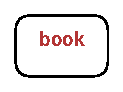
\includegraphics[scale=0.6]{gfx/text2kg/label.pdf}}}
			\Leftrightarrow
			\exists x: {\color{rot}label(x, \text{``book''})}
		\end{align}
	\item \textbf{$inst \subseteq \text{concept}^2$:}
		Die $inst$-Beziehung zwischen Konzepten entspricht grob der \textit{IS-A}-Beziehung semantischer Netze.
		Das Vorhandensein von $inst(x, y)$ impliziert, dass $prop(x) \subseteq prop(y)$ gilt;
		$inst$ ist also reflexiv und transitiv.
		\begin{align*}
			\textit{``the good book''}
			\Rightarrow
			\vcenter{\hbox{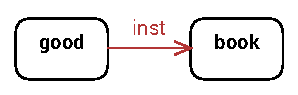
\includegraphics[scale=0.6]{gfx/text2kg/inst.pdf}}}
		\end{align*}
	\item \textbf{$relation \subseteq \text{concept}$:}
		Da die Prädikatsmenge eingeschränkt ist, können keine eigenen Prädikate für Worte eingeführt werden, die Konzepte in Relation zueinander setzen (z.~B. \textit{X likes Y}).
		Stattdessen werden sog.\ Relationskonzepte verwendet, d.~h.\ Konzepte, die andere Konzepte zueinander in Beziehung setzen.
		Relationskonzepte $r$ werden durch das unäre Prädikat $relation(r) \Leftrightarrow `relation \in prop(r)$ gekennzeichnet.
		Um die durch $r$ zueinander in Beziehung gesetzten Konzepte zu beschreiben werden die Prädikate $agent$ und $patient$ verwendet.
	\item \textbf{$agent \subseteq \text{concept}^2$:}
		Das $agent$-Prädikat zwischen einem Konzept $x$ und dem sog.\ Agens $y$ wird benutzt, um eine kausale Abhängigkeit des $x$ von $y$ zu beschreiben.
		$agent(x, y) \Leftrightarrow (`cause, y) \in prop(x)$ sagt also aus, dass $x$ aufgrund von $y$ existiert.
	\item \textbf{$patient \subseteq \text{concept}^2$:}
		Der Patiens $y$ eines Konzeptes $x$ ist ein Konzept, dessen Eigenschaften durch $x$ verändert werden.
		Es wird dabei davon ausgegangen, dass $x$ eine Eigenschaft $p_x \in prop(x)$ hat, die beschreibt, wie $x$ andere Konzepte verändert.
		$patient(x, y)$ impliziert, dass $prop(y)$ die durch $p_x$ geforderten Eigenschaften hat.
		$p_x$ lässt sich für natürlichsprachliche Konzepte offensichtlich nicht sinnvoll formal definieren.
		Dies ist allerdings auch nicht notwendig, wenn $p_x$ als von außen gegebenes Domänenwissen betrachtet wird, welches erst bei der Interpretation der Daten eingebracht wird.
\end{enumerate}
Diese Kombination von Prädikaten hat sich als hinreichend mächtig erwiesen, um eine Vielzahl natürlichsprachlicher Aussagen abzubilden.
\begin{align*}
	\textit{``I saw you yesterday.''}
	\Rightarrow
	\vcenter{\hbox{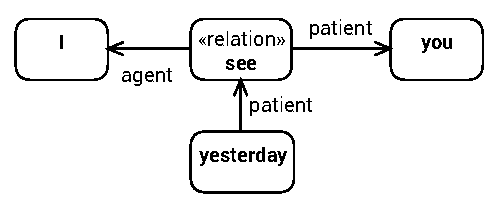
\includegraphics[scale=0.6]{gfx/text2kg/relAgPat.pdf}}}
\end{align*}

\subsection{Modale Kontexte}%
\label{sec:text2kg:ontology:modal}

Nachdem nun die verwendeten Prädikate beschrieben wurden, wird im zweiten Schritt geklärt, wie Wissensgraphen Modalität repräsentieren.
Beispiele für modale Aussagen sind:
\begin{center}
	\textit{``I {\color{blau}think} that {\color{rot}the book is good}.''}\\
	\textit{``{\color{rot}I} {\color{blau}don't want} to {\color{rot}see you}.''}
\end{center}
Die beiden Teilaussagen \textit{\color{rot}``the book is good''} und \textit{\color{rot}``I see you''} sind offensichtlich nicht unbedingt wahr, sondern beschreiben Möglichkeiten, die in Abhängigkeit von \textit{\color{blau}think} bzw.\ \textit{\color{blau}don't want} wahr oder falsch werden könnten.
Ob die Aussagen wahr werden, hängt davon ab, inwiefern das Denken oder Wollen einer Person mit der Realität --- auch aktuale Welt genannt --- übereinstimmt.
Dies ist je nach Person stark verschieden; manche tendieren dazu die allgemein als wahr akzeptierten Aussagen zu denken bzw.\ entsprechend ihrer Wünsche zu handeln, andere nicht.

Um derartige Möglichkeiten und Notwendigkeiten direkt zu repräsentieren, reichen die vorgestellten Konzeptgraphen mit Negationskontexten nicht aus.
Sowa hat dieses Problem ebenfalls erkannt und daher weitere Kontexttypen eingeführt.
Die Beschreibung dieser zusätzlichen Kontexttypen ist allerdings oftmals zu unpräzise für eine eindeutige Übersetzung in die Prädikatenlogik.
Aufbauend auf Sowas Ideen wird in dieser Arbeit daher eine Variante modaler Kontexte eingeführt, die die Übersetzbarkeit in die Prädikatenlogik erster Ordnung bewahrt.
Da die zuvor vorgestellten Konzeptgraphen bereits vollständig und korrekt sind, handelt es sich bei diesen modalen Kontexten also lediglich um eine Kurzschreibweise.

Insgesamt gibt es durch die Erweiterung um modale Kontexe nun folgende vier Kontexttypen:
\begin{multicols}{2}
	\flushleft\begin{enumerate}
		\item Positiver Aktualkontext
		\item Negativer Aktualkontext
		\item Positiver Möglichkeitskontext
		\item Negativer Möglichkeitskontext
	\end{enumerate}
\end{multicols}
Die modale Notwendigkeit hat keine eigenen Kontexttypen erhalten, um konsistent zur Quantisierung in Konzeptgraphen zu bleiben.
So, wie der Allquantor in Konzeptgraphen durch Negation der negierten existenzquantisierten Aussage ausgedrückt wird, wird die Notwendigkeit durch Negation der negativen Möglichkeit ausgedrückt.

Da es nun vier Kontexttypen gibt, muss die Konzeptgraphsyntax leicht angepasst werden, um zwischen den verschiedenen Typen differenzieren zu können:
\begin{figure}[h]
	\centering
	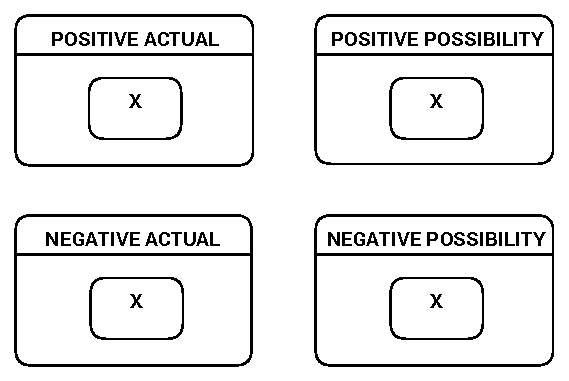
\includegraphics[scale=0.6]{gfx/text2kg/contextTypes.pdf}
	\caption{Konzeptgraphsyntax für modale Kontexte}\label{fig:text2kg:contextTypes}
\end{figure}

\paragraph{Positiver Aktualkontext}
Dieser Kontexttyp hat keinen Einfluss auf die Bedeutung der enthaltenen Knoten.
Er entspricht in etwa der Klammerung in der Prädikatenlogik.
Das \textit{Sheet of Assertion}~$\top$ ist ein solcher Kontext, abgesehen davon tauchen positive Aktualkontexte allerdings nicht auf;
sie werden hier lediglich der Vollständigkeit halber erwähnt.
\begin{align}
	\vcenter{\hbox{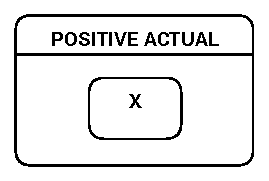
\includegraphics[scale=0.6]{gfx/text2kg/positiveActual.pdf}}}
	\Leftrightarrow
	\vcenter{\hbox{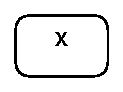
\includegraphics[scale=0.6]{gfx/text2kg/x.pdf}}}
	\Leftrightarrow
	\exists x: label(x, \text{``X''})
\end{align}

\paragraph{Negativer Aktualkontext}
Entspricht dem bisherigen Negationskontext.
\begin{align}
	\vcenter{\hbox{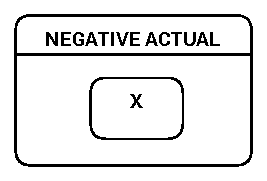
\includegraphics[scale=0.6]{gfx/text2kg/negativeActual.pdf}}}
	\Leftrightarrow
	\lnot \exists x: label(x, \text{``X''})
\end{align}

\paragraph{Positiver Möglichkeitskontext}
Dieser Kontexttyp bildet die modale Möglichkeit ab.
Um die Mächtigkeit der Prädikatenlogik beizubehalten, wird hierfür keine fundamental neue Struktur eingeführt.
Es wird stattdessen die Tatsache ausgenutzt, dass sich die modalen Operatoren gemäß der Mögliche-Welten-Interpretation analog zu den prädikatenlogischen Quantoren verhalten.
\begin{align*}
	{\color{rot}\square} P(x)\ &\Leftrightarrow \lnot {\color{blau}\lozenge} \lnot P(x) \\
	{\color{rot}\forall} w: world(w) \rightarrow P_w(x)\ &\Leftrightarrow \lnot {\color{blau}\exists} w: world(w) \land \lnot P_w(x) \numberthis
\end{align*}
Die Aussage \textit{``$P(x)$ gilt notwendigerweise''}, wird also als \textit{``Es gibt keine Welt $w$ in der $P_w(x)$ nicht gilt''} aufgefasst.
Statt von Welten, wird in modalen Konzeptgraphen allerdings von Kontexten gesprochen.
\begin{align*}
	\vcenter{\hbox{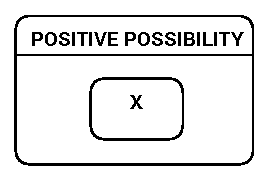
\includegraphics[scale=0.6]{gfx/text2kg/positivePossib.pdf}}}
	&\Leftrightarrow
	\vcenter{\hbox{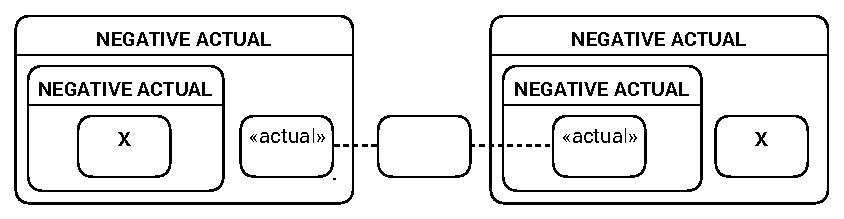
\includegraphics[scale=0.6]{gfx/text2kg/possibExpansion.pdf}}} \numberthis \\
	&\Leftrightarrow
	\exists c: context(c) \land (actual(c) \leftrightarrow \exists x: label(x, \text{``X''}))
\end{align*}
Anders als Aktualkontexte, tauchen Möglichkeitskontexte explizit in der prädikatenlogischen Repräsentation auf, sie lassen sich also nicht nur als Kontext sondern zugleich auch als Konzept auffassen.
Der in einem Möglichkeitskontext $c$ enthaltene Teilgraph $G$ ist dabei genau dann wahr, wenn der Kontext die aktuale Welt beschreibt~($\Leftrightarrow actual(c)$).
Solange $actual(c)$ unbekannt ist, kann also keine Aussage über die Wahrheit von $G$ gemacht werden.
Wenn $actual(c)$ jedoch wahr bzw.\ falsch ist, ist $c$ äquivalent zu einem positiven bzw.\ negativen Aktualkontext.

Zur Bestimmung von des Wahrheitswertes von $actual(c)$ ist i.~d.~R. domänenspezifisches Wissen notwendig.
Dieses domänenspezifische Wissen, kann durch sog.\ Kontextrelationen eingebracht werden.
Da Möglichkeitskontexte zugleich Konzepte sind, lassen sie sich zu anderen Konzepten in Relation setzen.
Dies ist z.~B. dann nützlich, wenn man die Aussage \textit{``I {\color{blau}think} that {\color{rot}the book is good}.''} repräsentieren möchte.
\begin{align*}
	&\vcenter{\hbox{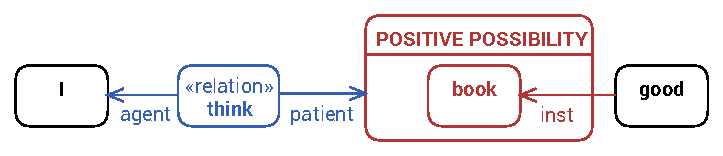
\includegraphics[scale=0.6]{gfx/text2kg/possibCtxRelationExample.pdf}}} \numberthis \\
	\Leftrightarrow
	\exists i, g, t, c:&\ label(i, \text{``I''}) \land label(g, \text{``good''}) \\
	\land&\ {\color{blau}label(t, \text{``think''}) \land relation(t) \land agent(t, i) \land patient(t, c)} \\
	\land&\ {\color{rot}context(c) \land (actual(c) \leftrightarrow \exists b: label(b, \text{``book''}) \land inst(g, b))}
\end{align*}
Durch die Verknüpfung $patient(t, c)$ eines Konzeptes mit einem Kontext, kann Wissen über das Konzept benutzt werden, um Schlüsse über die Aktualität des Kontextes zu ziehen.
Wie genau dies ablaufen kann, ist bislang allerdings noch unklar.
In \treft{sec:text2kg:psl} wird die $actual$-Inferenz näher untersucht.

\paragraph{Negativer Möglichkeitskontext}
Lediglich eine Kurzschreibweise für einen positiven Möglichkeitskontext der einen negativen Aktualkontext umgibt.
\begin{align}
	\vcenter{\hbox{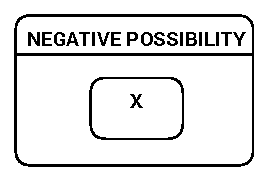
\includegraphics[scale=0.6]{gfx/text2kg/negativePossib.pdf}}}
	\Leftrightarrow
	\vcenter{\hbox{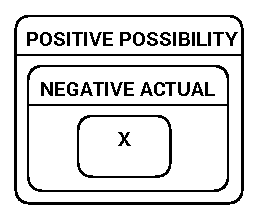
\includegraphics[scale=0.6]{gfx/text2kg/negativePossibExpansion.pdf}}}
\end{align}

\section{NLP-Phase}%
\label{sec:text2kg:nlp}

In diesem Abschnitt werden die ersten beiden Stufen der Konstruktionspipeline beschrieben.
Die erste Stufe ist im Wesentlichen lediglich ein Wrapper um verschiedene CoreNLP-Annotatoren.
In der zweiten Stufe werden dann die CoreNLP-Annotationen in einen Konzeptgraphen mit der soeben beschriebenen Ontologie transformiert.
\begin{figure}[h]
	\centering
	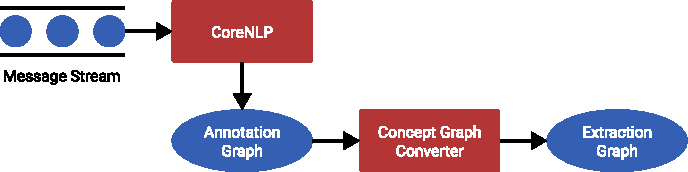
\includegraphics[width=0.67\textwidth]{gfx/text2kg/nlpPhase.pdf}
	\caption{NLP-Phase der Konstruktionspipeline}\label{fig:text2kg:nlpPhase}
\end{figure}

\subsection{Nachrichtenformat}%
\label{sec:text2kg:nlp:msg}

Vor der Beschreibung der Pipeline-Stufen, muss geklärt werden, wie genau die eingegebenen Nachrichten aufgebaut sind.
Da diese Arbeit lediglich die grundlegende Architektur eines Wissensgraphkonstruktionsverfahrens beschreibt, wurde eine vereinfachte Struktur gewählt, die die wesentlichen Eigenschaften von Nachrichten enthält.
Eine Nachricht wird daher im Folgenden als ein Tupel mit den folgenden Komponenten verstanden:
\begin{enumerate}
	\item \textbf{Sender:}
		Als Sender wird, der Einfachheit halber, der Name des Absenders verwendet.
		Im Kontext von E-Mail Nachrichten müsste zwar zwischen dem Absendernamen und der Absenderadresse differenziert werden, diese Unterscheidung macht das Verfahren allerdings lediglich komplizierter, ohne dabei die Kernaspekte zu bereichern.
	\item \textbf{Empfänger:}
		Auch hier wird lediglich der Empfängername benutzt.
		Nachrichten mit mehreren Empfängern werden in dieser Arbeit nicht betrachtet.
	\item \textbf{Sendedatum:}
		Gemeint ist hiermit lediglich ein Datum der Form \texttt{YYYY-MM-DD}.
		Uhrzeiten und Zeitzonen werden nicht berücksichtigt.
	\item \textbf{Inhalt:}
		Der Nachrichteninhalt wird als natürlichsprachliche Zeichenkette verstanden.
		Als Sprache wird dabei Englisch angenommen, da CoreNLP dann die besten Ergebnisse liefert.
		Zudem werden eingebundene Multimedia-Inhalte und Anhänge nicht berücksichtigt.
\end{enumerate}

Zwei sehr einfache exemplarische Nachrichten sind:
\begin{center}\pbox{\textwidth}{
	$(m_1)$ \texttt{2017-06-11}: Bob $\rightarrow$ Alice: \textit{``I think I saw you today.''} \\ % chktex 8
	$(m_2)$ \texttt{2017-06-12}: Alice $\rightarrow$ Bob: \textit{``I don't think I saw you yesterday.''} % chktex 8
}\end{center}

\subsection{CoreNLP Annotation}%
\label{sec:text2kg:nlp:corenlp}

In \treft{sec:theory:nlp} wurden die, für diese Arbeit wesentlichen, Annotatoren bereits vorgestellt: Tokenization, Lemmatization, POS-Tagging, NER, Coreference Resolution und Dependency Parsing.
Um mit den Ergebnissen all dieser Annotatoren zu arbeiten, werden jene in einer gemeinsamen Datenstruktur zusammengefasst, dem sog.\ \textit{Annotationsgraphen}.
Hierbei handelt es sich um den Abhängigkeitsgraphen des Dependency Parsers, in den die Ergebnisse der anderen Annotatoren eingefügt wurden:
\begin{enumerate}
	\item \textbf{Lemmata:}
		Die Vollformen der Token werden durch ihre Lemmata ersetzt.
		Dieser Änderung liegt die Annahme zugrunde, dass die syntaktische Repräsentation einer Wortbeugung i.~d.~R. nicht relevant ist.
		Durch die Lemmatisierung wird es einfacher ähnliche Begriffe aufgrund ihrer textuellen Ähnlichkeit zu identifizieren.
	\item \textbf{POS-Tags:}
		Durch das Verwerfen der Token-Vollformen können wertvolle grammatikalische Informationen verloren gehen.
		Daher wird jedem Token-Knoten sein POS-Tag hinzugefügt, welcher die Wortart und Beugung jedes lemmatisierten Tokens einheitlich repräsentiert.
	\item \textbf{NER-Klassen:}
		Alle Token-Knoten, die der NER-Annotator klassifizieren konnte, erhalten ihre Klasse und im Fall von numerischen oder Datums-Token eine normalisierte Form des Wertes, den sie repräsentieren.
	\item \textbf{Koreferenzklassen:}
		Jede gefundene Token-Koreferenzklasse $C = \{t_1, \dots, t_n\}$ wird als eine Menge von Koreferenzkanten in den Annotatinsgraphen eingefügt.
		Als Kantenmenge wird allerdings nicht $C \times C$ verwendet, da diese unnötig groß ist und zudem nicht alle verfügbaren Informationen repräsentiert.
		Die CoreNLP Coreference Resolution ordnet jeder Klasse nämlich eine sog.\ \textit{Representative Mention} $rep(C) \in C$ zu.
		$rep(C)$ ist das Token einer Klasse, welches diese am besten repräsentiert.
		\begin{align*}
			\text{T}\tikzmark{toma}\text{om is calling hi}\tikzmark{tomb}\text{s brother.}
			\begin{tikzpicture}[overlay,remember picture]
				\draw[-,shorten >=3pt,shorten <=3pt] (toma.center) to[bend right] (tomb.center);
			\end{tikzpicture}
			\Rightarrow
			C = \{\text{Tom}, \text{his}\}, rep(C) = \text{Tom}
		\end{align*}
		Um die $rep$-Information zu erhalten, werden nur Koreferenzkanten von $rep(C)$ zu den anderen Klassentoken $C \setminus \{rep(C)\}$ hinzugefügt.
\end{enumerate}

\subsection{Konzeptgraphtransformation}%
\label{sec:text2kg:nlp:transform}

\section{Wissensgraphkonstruktionsphase}%
\label{sec:text2kg:psl}
